\documentclass[11pt]{article}

\usepackage{a4wide}
\usepackage{amsmath}
\usepackage{natbib}
\usepackage{booktabs}
\usepackage{graphicx}
\usepackage{tabularx}
%\graphicspath{{expt/}}
\usepackage{times}
\usepackage[varg]{txfonts}
\usepackage{color}
\usepackage{epsfig}
\usepackage{verbatim}
\usepackage[hidelinks]{hyperref}
\usepackage{enumitem}

\begin{document}

\pagenumbering{arabic}
\title{TN2624 MATLAB Session 11\\Solutions}
\date{May 23, 2013}
%\date{\today}
\maketitle


%%%%%%%%%%%%%%%%%%%%%%%%%%%%%%%%%%%%%%%%%%%%%%%%%%%%%%%%
%%%%%%%%%%%%%%%%%%%%%%%%%%%%%%%%%%%%%%%%%%%%%%%%%%%%%%%%
%%%%%%%%%%%%%%%%%%%%%%%%%%%%%%%%%%%%%%%%%%%%%%%%%%%%%%%%

\section*{Semiconductor statistics Part 1  -- the intrinsic semiconductor (70 pts)}
\label{sec:lot}

\begin{enumerate}[resume]
\item \textbf{(25 pts)} Fermi-Dirac distribution and density of states as a function of energy.\\
\begin{figure}[h]
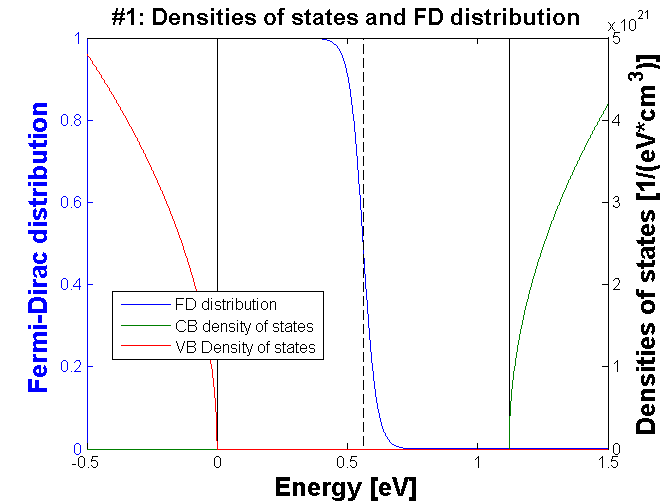
\includegraphics[width=0.6\textwidth]{F1.png}
\end{figure}

\item \label{itm:occhole} \textbf{(5 pts)} The same as the distribution for the electrons, but mirrored at the chemical potential
$$ \bar {n}_\text{FD,h}(E)=\frac{1}{1+\exp{\frac{\mu-E}{k T}}}.$$ 

\item \label{itm:aa}\textbf{(10 pts)} 

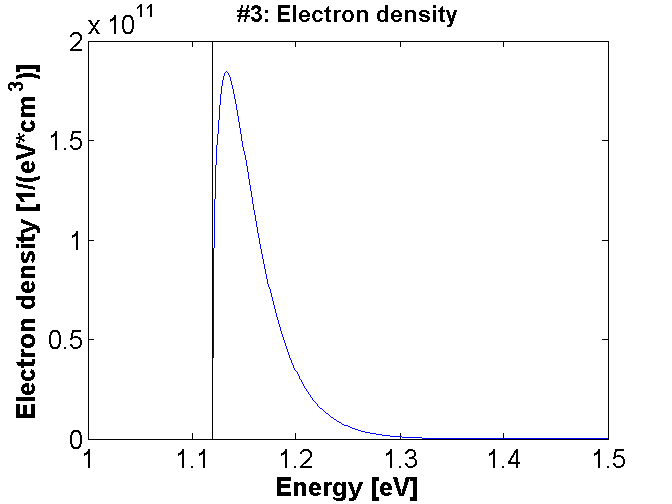
\includegraphics[width=0.6\textwidth]{F3.png}


\item \textbf{(5 pts)} \verb|%Result: 9.8506e+09 1/cm^3|, way too low

\item \label{itm:tempdep}\textbf{(25 pts)} 

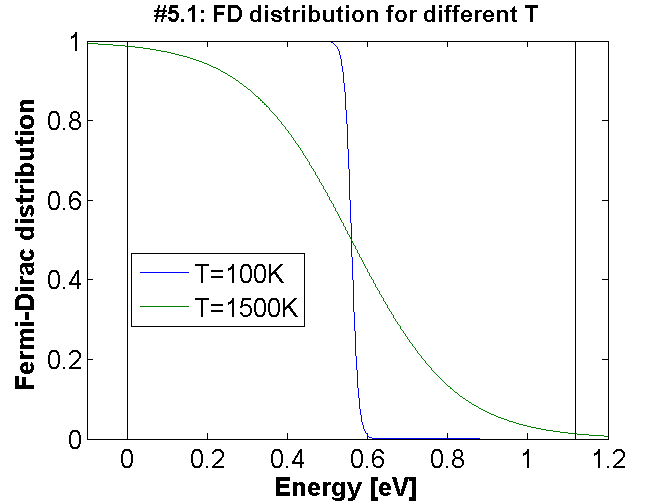
\includegraphics[width=0.45\textwidth]{F5_1.png}
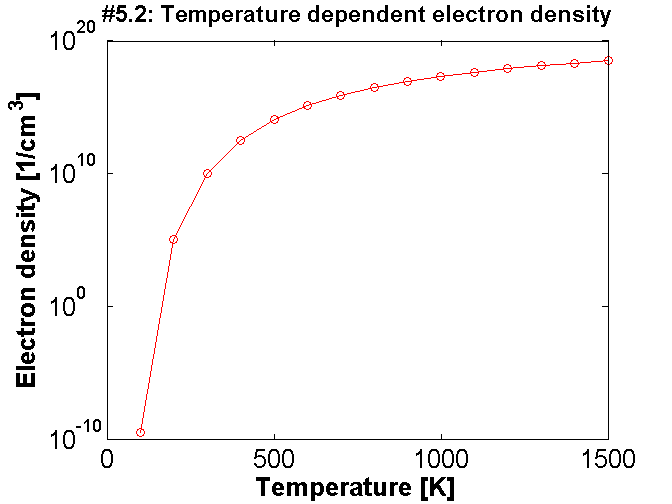
\includegraphics[width=0.45\textwidth]{F5_2.png}
Fermi-Dirac distribution ``smears out'' at higher temperatures $\rightarrow$ more electrons excited to the conduction band\\
Unrealistically high temperatures would be required to obtain significant electron densities

\section*{Semiconductor statistics Part 2 -- the doped semiconductor (30 pts)}
\label{sec:lot}

\item \textbf{(20 pts)}\\ \verb|mu=1.0300 %eV|,\\ \verb|n=7.6210e+17 %cm^-3|,\\ \verb|p=125.9659 %cm^-3|, virtually no holes in the valence band... all electrons stem from the dopants

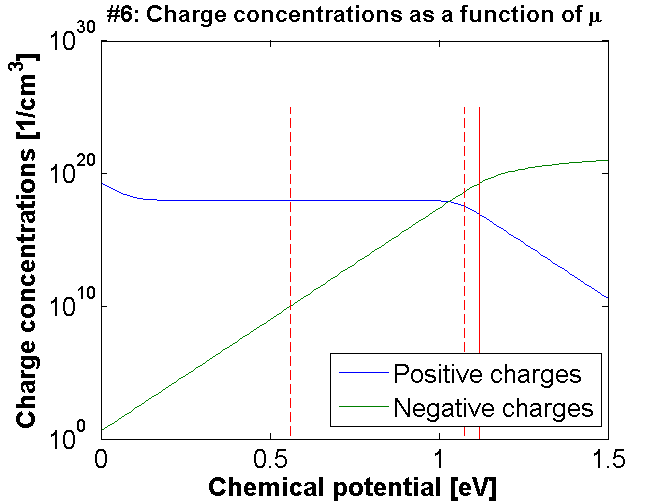
\includegraphics[width=0.6\textwidth]{F6.png}

\item \textbf{(10 pts)} \\
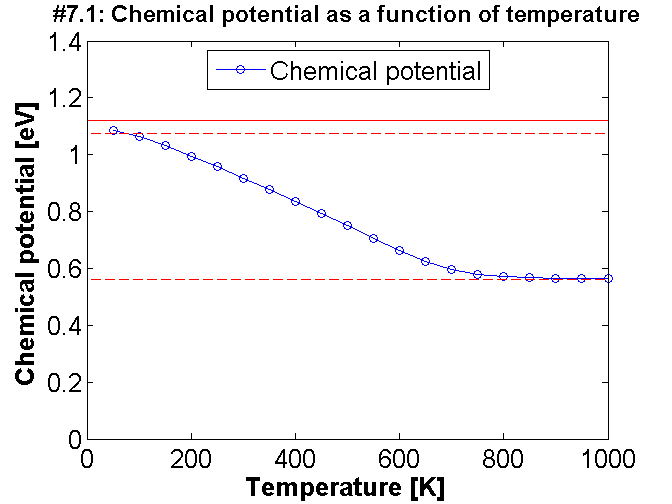
\includegraphics[width=0.45\textwidth]{F7_1.png}
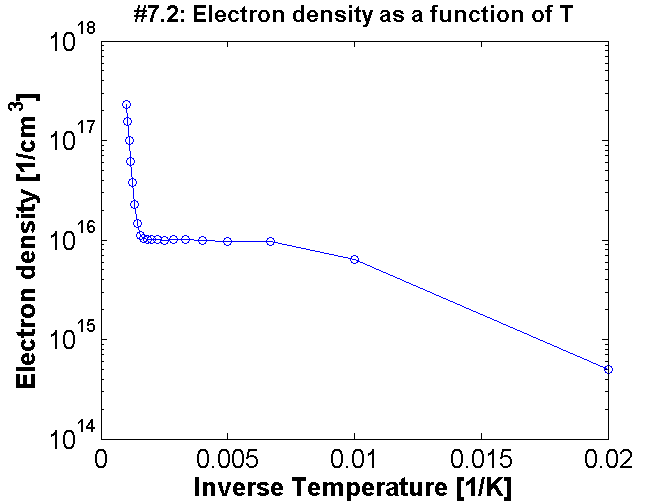
\includegraphics[width=0.45\textwidth]{F7_2.png}

\begin{itemize}
\item Low temperature: The electrons from the dopants get excited to the conduction band
\item Medium temperature: All the dopants have been activated (electron density saturates to dopant density), yet the temperature is still too low to excite electrons from the valence band to the conduction band
\item High temperature: Electrons can be excited from the valence band to the conduction band
\end{itemize}




\end{enumerate}



















\end{document}